%!TEX root = main.tex

\section{Necessary Conditions}
We begin with two results that focus on the structure of the equality constraints.
\begin{theorem}[Geometric Necessary Condition for Linear Equality Constraints]\index{Theorem!Geometric necessary condition}
If $(P)$ is a consistent program with linear equality constraints $h_k(\x) = \langle \boldsymbol{a}_k, \x \rangle + b_k$ ($\boldsymbol{a}_k \in \field{R}^d$, $b_k \in \field{R}$) for all $1 \leq k \leq \ell$, then for all feasible local minima $\x \in S$,
\begin{equation*}
\mathcal{F}_0(\x) \cap \mathcal{G}_0(\x) \cap \mathcal{H}_0(\x) = \emptyset.
\end{equation*}
\end{theorem}

\begin{theorem}[Geometric Necessary Condition for Linearly Independent Equality Constraints]\index{Theorem!Geometric necessary condition}
If $\x \in S$ is a feasible local minimum for the consistent program $(P)$, and the gradient vectors $\{ \gradient{h_k}(\x) : 1 \leq k \leq \ell \}$ are linearly independent, then $\mathcal{F}_0(\x) \cap \mathcal{G}_0(\x) \cap \mathcal{H}_0(\x) = \emptyset$.
\end{theorem}

\separator

As a consequence, an algebraic version of this geometric necessary condition gives the following result.

\begin{theorem}[Fritz John Necessary Conditions]\index{Theorem!Fritz John necessary conditions}
If $\x \in S$ is a feasible local minimum of the consistent program $(P)$, then there exist $u_k \geq 0$ for $0\leq k \leq m$, and $v_1, \dots, v_\ell \in \field{R}$ so that
\begin{enumerate}
 	\item $[u_0, u_1, \dotsc, u_m, v_1 \dotsc, v_\ell ] \neq \boldsymbol{0}$,
 	\item $u_k g_k(\x) = 0$ for all $1 \leq k \leq m$.
 	\item $u_0 \gradient{f}(\x) + \sum_{k=1}^m u_k \gradient{g_k}(\x) + \sum_{k=1}^\ell v_k \gradient{h_k}(\x) = 0$.
 \end{enumerate}
\end{theorem}

\begin{theorem}[Karush-Kuhn-Tucker Necessary Conditions]\index{Theorem!Karush-Kuhn-Tucker}\index{Theorem!KKT necessary conditions}\label{theorem:KKTnecessary}
If $\x \in S$ is a feasible local minimum of the consistent program $(P)$ for which all the vectors $\{ \gradient{h_k}(\x), \gradient{g_j}(\x) : 1 \leq k \leq \ell, j \in \mathcal{I}(\x) \}$ are linearly independent, then there exist $u_k \geq 0$ for $1\leq k \leq m$, and $v_1, \dots, v_\ell \in \field{R}$ so that
\begin{enumerate}
 	\item $[u_0, u_1, \dotsc, u_m, v_1 \dotsc, v_\ell ] \neq \boldsymbol{0}$,
 	\item $u_k g_k(\x) = 0$ for all $1 \leq k \leq m$.
 	\item $u_0 \gradient{f}(\x) + \sum_{k=1}^m u_k \gradient{g_k}(\x) + \sum_{k=1}^\ell v_k \gradient{h_k}(\x) = 0$.
 \end{enumerate}
\end{theorem}

\begin{example}
Continuing with example \ref{example:feasibleP1}, let's check if the point $(0,0)$ is a candidate to optimal solution of this program.  Let's use Theorem \ref{theorem:KKTnecessary} to verify this claim:
\begin{align*}
\gradient{f}(x,y) &= [ 4x^3, 4y^3 ] &\gradient{f}(0,0) &= [0,0], \\
\gradient{g_1}(x,y) &= [ 2x, 0 ] &\gradient{g_1}(0,0) &= [0,0], \\
\gradient{g_2}(x,y) &= [0, 2y] &\gradient{g_2}(0,0) &= [0,0], \\
\gradient{g_3}(x,y) &= \big[e^{x+y}, e^{x+y} \big] &\gradient{g_3}(0,0) &= [1,1].
\end{align*}
Notice how the gradients \emph{line up} nicely---can we find $u_k \geq 0$ (not all of them simultanously equal to zero) so that the following linear combination is equal to $[0,0]$?
\begin{gather*}
\gradient{f}(0,0) + u_1 \gradient{g_1}(0,0) + u_2 \gradient{g_2}(0,0) + u_3 \gradient{g_3}(0,0) = [0,0], \\
[0,0] + u_1[0,0] + u_2[0,0] +u_3[1,1] = [0,0],
\end{gather*}
We may select, for instance $u_1=u_2=1$, $u_3=0$, which proves that the point $(0,0)$ is indeed a candidate for optimal solution of $(P)$.
\end{example}


\begin{example}\label{example:feasibleP3}
Set $f(x,y)=(x-12)^2+(y+6)^2$.  Consider the program $(P)$ designed to find the global minimum of this function on the set $S=\{ (x,y) \in \field{R}^2 : x^2+3x+y^2-4.5y \leq 6.5, (x-9)^2 +y^2 \leq 64, 8x+4y=20 \}$.  We want to prove that the point $(2,1)$ is a good candidate for optimal solution of $(P)$.
The point $(2,1)$ is feasible.  To see this, set 
\begin{align*}
g_1(x,y) &=x^2+3x+y^2-4.5y-6.5, \\
g_2(x,y) &=(x-9)^2+y^2-64, \\
h_1(x,y) &=8x+4y-20,
\end{align*}
(or simpler equivalent constraints), and notice that
\begin{equation*}
g_1(2,1)=-12, \quad g_2(2,1)=-14, \quad h_1(2,1)=0.
\end{equation*}
\begin{figure}[ht!]
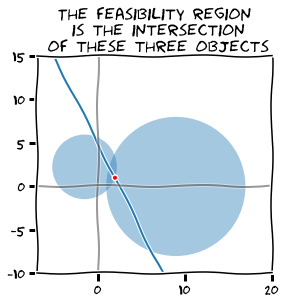
\includegraphics[width=0.5\linewidth]{images/feasibleP3.png}
\caption{Feasibility region for $(P)$ in example \ref{example:feasibleP3}}
\label{figure:feasibleP3}
\end{figure}
We have concluded that $(P)$ is consistent.  To verify that $(2,1)$ is candidate for optimal solution of $(P)$, we may now use Theorem \ref{theorem:KKTnecessary} and check if the gradients line up nicely for this point:
\begin{align*}
\gradient{f}(x,y)   &= [ 2(x-12), 2(y+6) ] &\gradient{f}(2,1)   &= [-20, 14], \\
\gradient{g_1}(x,y) &= [ 2x+3, 2y-4.5 ]    &\gradient{g_1}(2,1) &= [  7, -2.5], \\
\gradient{g_2}(x,y) &= [ 2(x-9), 2y ]      &\gradient{g_2}(2,1) &= [-14, 2], \\
\gradient{h_1}(x,y) &= [ 8, 4]             &\gradient{h_1}(2,1) &= [  8, 4], 
\end{align*}
Looking for $u_k \geq 0, v_1 \in \field{R}$ (not all of them simultaneously equal to zero) so that the following linear combination is equal to $[0,0]$.
\begin{align*}
\gradient{f}(2,1) + u_1 \gradient{g_1}(2,1) + u_2 \gradient{g_2}(2,1) + v_1 \gradient{h_1}(2,1) &= [0,0], \\
[-20,14] + u_1 [7,-2.5] + u_2 [-14,2] + v_1 [8,4] = [0,0]
\end{align*}
or equivalently
\begin{equation*}
\begin{bmatrix} 7 & -14 \\ -2.5 & 2 \end{bmatrix} \begin{bmatrix} u_1 \\ u_2 \end{bmatrix} = \begin{bmatrix} 20 - 8v_1 \\ -14-4v_1 \end{bmatrix}
\end{equation*}
Among all possible solutions, pick for instance $u_1=4$, $u_2=0$ and $v_1=-1$ to prove that the point $(2,1)$ is indeed a good candidate for the optimal solution of $(P)$.
\end{example}
